% !TEX encoding = UTF-8 Unicode 
% !TEX root = on_gates.tex

\clearpage


\section{Clifford Gates}

The Clifford gates are an important subgroup of quantum gates. Familiar examples include the Pauli gates (I, X, Y, Z), phase (S), Hadamard (H), controlled-Z (CZ), controlled-not (CNOT), and swap.  Common non-Clifford gates include T, B, and Toffolli (CCNOT). 

The {\sl Clifford group}  $C_n$ of gates acting on $n$ qubits consists of those gates that {\sl normalize} the corresponding Pauli group $P_n$. In the context of groups, {\sl normalize} means that if $p$ is an element of the Pauli group, and $V$ is a Clifford gate, then $p' = V p V^\dagger$ is also an element of the Pauli group.
\[
\mathbf{C}_n=\{V\in U_{2^n}\mid V\mathbf{P}_nV^\dagger = \mathbf{P}_n\}
\]
% TODO PHASE, quotient group.

The Clifford gates are defined this way because of important applications in quantum  error correcting, which we will come to presently.
An alternative approach is to define the Clifford group as all gates that can be constructed from S, H, and CNOT. This is the same group, up to phase. 
% The definition of the Clifford group as the normalizer of the Pauli group may appear to be somewhat esoteric at first. 


\subsection{Single qubit Clifford gates}
Consider the X gate as a Clifford acting on  the $X$, $Y$, and $Z$ single-qubit Pauli elements. 
\[
XXX^\dagger &= 
	\begin{bsmallmatrix}0 & 1 \\ 1 & 0 \end{bsmallmatrix}
	\begin{bsmallmatrix}0 & 1 \\ 1 & 0 \end{bsmallmatrix}
	\begin{bsmallmatrix}0 & 1 \\ 1 & 0 \end{bsmallmatrix}
	= \begin{bsmallmatrix}0 & 1 \\ 1 & 0 \end{bsmallmatrix}
    = +X 
\notag \\
XYX^\dagger &=
	\begin{bsmallmatrix}0 & 1 \\ 1 & 0 \end{bsmallmatrix}
	\begin{bsmallmatrix}0 & -i \\ i & 0 \end{bsmallmatrix}
	\begin{bsmallmatrix}0 & 1 \\ 1 & 0 \end{bsmallmatrix}
	= \begin{bsmallmatrix}1 & 0 \\ 0 & -1 \end{bsmallmatrix}
    = -Z
\notag \\ 
XZX^\dagger
& =	\begin{bsmallmatrix}0 & 1 \\ 1 & 0 \end{bsmallmatrix}
	\begin{bsmallmatrix}1 & 0 \\ 0 & -1 \end{bsmallmatrix}
	\begin{bsmallmatrix}0 & 1 \\ 1 & 0 \end{bsmallmatrix} 
	= \begin{bsmallmatrix}0 & -i \\ i & 0 \end{bsmallmatrix}
    = -Y
\notag
\]

Or the Hadamard gate
\[
HXH^\dagger &= \tfrac{1}{2}
	\begin{bsmallmatrix}1 & -1 \\ 1 & 1 \end{bsmallmatrix}
	\begin{bsmallmatrix}0 & 1 \\ 1 & 0 \end{bsmallmatrix}
	\begin{bsmallmatrix}1 & -1 \\ 1 & 1 \end{bsmallmatrix}
	= 	\begin{bsmallmatrix}1 & 0 \\ 0 & -1 \end{bsmallmatrix}
    = +Z
\notag \\
HYH^\dagger &= \tfrac{1}{2}
	[\begin{smallmatrix}1 & -1 \\ 1 & 1 \end{smallmatrix}]
	[\begin{smallmatrix}0 & -i \\ i & 0 \end{smallmatrix}]
	[\begin{smallmatrix}1 & -1 \\ 1 & 1 \end{smallmatrix}]
	= 	[\begin{smallmatrix}0 & i \\ -i & 0 \end{smallmatrix}]
    = -Y
\notag \\ 
HZH^\dagger & =\tfrac{1}{2}
		\begin{bsmallmatrix*}[r]1 & -1 \\ 1 & 1 \end{bsmallmatrix*}
		\begin{bsmallmatrix*}[r] 1 & 0 \\ 0 & -1 \end{bsmallmatrix*}
		\begin{bsmallmatrix*}[r] 1 & -1 \\ 1 & 1 \end{bsmallmatrix*}
	= 	\begin{bsmallmatrix*}[r] 0 & 1 \\ 1 & 0 \end{bsmallmatrix*}
    = +X
\notag
\]
Note that we only ever pick up a $\pm 1$ phase, and never an imaginary phase. This is because any element of the Pauli group  with $\pm 1$ phase is Hermitian, and the transformed gate $U p U^\dagger$ must also Hermitian. Therefore we can't pick up an imaginary phase. 

On the other hand, if we look at these transformations for a non-Clifford gate such as the $T$ gate, we do not recover Pauli elements.
\[
TXT^\dagger &= 
	[\begin{smallmatrix}1 & 0 \\ 0 & e^{+i\frac{\pi}{4}} \end{smallmatrix}]
	[\begin{smallmatrix}0 & 1 \\ 1 & 0 \end{smallmatrix}]
	[\begin{smallmatrix}1 & 0 \\ 0 & e^{-i\frac{\pi}{4}} \end{smallmatrix}]
	= 	[\begin{smallmatrix}0 & e^{+i\frac{\pi}{4}} \\ e^{-i\frac{\pi}{4}} & 0 \end{smallmatrix}]
\notag \\
TYT^\dagger &= 
	[\begin{smallmatrix}1 & 0 \\ 0 & e^{+i\frac{\pi}{4}} \end{smallmatrix}]
	[\begin{smallmatrix}0 & -i \\ i & 0 \end{smallmatrix}]
	[\begin{smallmatrix}1 & 0 \\ 0 & e^{-i\frac{\pi}{4}} \end{smallmatrix}]
	= 	-[\begin{smallmatrix}0 & e^{+i\frac{\pi}{4}} \\ e^{-i\frac{\pi}{4}} & 0 \end{smallmatrix}]
\notag \\ 
TZT^\dagger & =
		[\begin{smallmatrix}1 & 0 \\ 0 & e^{+i\frac{\pi}{4}} \end{smallmatrix}] 
		[\begin{smallmatrix}1 & 0 \\ 0 & -1 \end{smallmatrix}]
		[\begin{smallmatrix}1 & 0 \\ 0 & e^{-i\frac{\pi}{4}} \end{smallmatrix}]
	= 	[\begin{smallmatrix}1 & 0 \\ 0 & -1 \end{smallmatrix}] = Z
\notag
\] 



Up to phase, a Clifford gate is completely determined by its transformation of the Pauli elements [TODO: Why?]. And because the Pauli group elements are tensor products acting independently on separate qubits, we need only consider the action of the Clifford group on each of the $4n$ single qubit Pauli gates. Moreover, the action of the identity is trivial, and the action on $Y$ can be determined by that on $X$ and $Y$, since $VYV^\dagger= -i VXZV^\dagger = -i\ VXV^\dagger\ VZV^\dagger$. For single qubit Cliffords, $X$ can map to 6 possibilities, $\{\pm X, \pm Y, \pm Z\}$,  leaving 4 possibilities for the action on $Z$. This gives a total of $6\times4=24$ distinct 1-qubit Clifford groups. 

The 24 1-qubit Clifford gates are isomorphic to the group of rotations of an octahedron.  The coordinates $R_n(\theta)$ of these are listed in table ???, along with the Pauli mappings.
 If we think of the Pauli gates $X$, $Y$, $Z$ as the 3 cartesian axes $x, y, z$, then the elements of the Clifford group correspond to rotations that map axes to axes. We have 3 elements that rotate 180$^{\circ}$ about vertices (X, Y, Z); 6 elements (the square roots of $X$, $Y$, and $Z$) that rotate 90$^{\circ}$ or 270$^{\circ}$ degrees around vertices; 6 Hadamard like gates that rotate 180$^{\circ}$ about edges; another 8 gates that rotation 120$^{\circ}$ or 240$^{\circ}$ degrees around faces; and the identity. This is a subgroup of the full octahedral group (which includes inversions), and also equal(??) to $S_4$, the group of permutations of 4 objects.
 \index{Hadamard-like gates} \index{octahedral group}\index{permutation group}

\begin{center}
 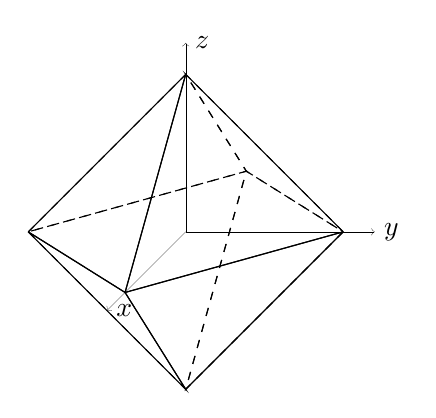
\begin{tikzpicture}[scale=2]

\draw[ultra thin, ->] (0,0,0) -- (0, 0, 1.3) node[right] {$x$};
\draw[ultra thin, ->] (0,0,0) -- (0, 1.2, 0) node[right] {$z$};
\draw[ultra thin, ->] (0,0,0) -- (1.2, 0, 0) node[right] {$y$};


\draw (1, 0, 0) -- (0, 1, 0) -- (0, 0, 1) -- (1, 0, 0);
\draw[dashed] (1, 0, 0) -- (0, 1, 0) -- (0, 0, -1) -- (1, 0, 0);
\draw (1, 0, 0) -- (0, -1, 0) -- (0, 0, 1) -- (1, 0, 0);
\draw[dashed] (1, 0, 0) -- (0, -1, 0) -- (0, 0, -1) -- (1, 0, 0);

\draw (-1, 0, 0) -- (0, 1, 0) -- (0, 0, 1) -- (-1, 0, 0);
\draw[dashed] (-1, 0, 0) -- (0, 1, 0) -- (0, 0, -1) -- (-1, 0, 0);
\draw (-1, 0, 0) -- (0, -1, 0) -- (0, 0, 1) -- (-1, 0, 0);
\draw[dashed] (-1, 0, 0) -- (0, -1, 0) -- (0, 0, -1) -- (-1, 0, 0);

 \end{tikzpicture}
 \end{center}


All 24 single qubit Clifford gates can be generated from just 2 elements, traditionally chosen to be $S$ and $H$. For instance $X=HSSH$. Since  $(S H)^3 = e^{2\pi i/8} I$ we can generate each Clifford gate with 8 different phases. This is why you'll sometimes see the number of 1-qubit Clifford gates reported as $8\times24=192$, which includes in the possible Clifford gates integers powers of a phase $\omega^k = e^{2\pi i k/8}$, $k ={0,1,\ldots,7}$.



\begin{table}[htp]
\caption{Coordinates of the 24 1-qubit Clifford gates.}
\label{tab:Clifford1q}
\begin{center}
\begin{tabular}{crrrrrrrcc}
Gate & $\theta$ & $n_x$ & $n_y$ & $n_z$ &~~~~  $X$ & $Y$ & $Z$ \\
\\
$I$ & 0 &&&												& $+X$ & $+Y$ & $+Z$
\\ \\
$V$ 					& $\sfrac{1}{2}\pi$ 	& 1 & 0 & 0 & $+X$ & $?Z$ & $+Y$  
\\
$X$ 					& $\pi$ 				& 1 & 0 & 0 & $+X$ & $-Y$ & $-Z$  %&  $H\ Z\ H$
\\
$ V^\dagger$   			& $-\sfrac{1}{2}\pi$ 	& 1 & 0 & 0 &%&  $H\ S^\dagger H$
\\
$h^\dagger$            	& $\sfrac{1}{2}\pi$ 	& 0 & 1 & 0 &%&  $S^\dagger H\ S\ H\ S$
\\
$Y$ 			      	& $\pi$ 		 		& 0 & 1 & 0 &%&  $S^\dagger H\ Z\ H\ S$
\\
$h$    					& $-\sfrac{1}{2}\pi$  	& 0 & 1 & 0 &%&  $S^\dagger H\ S^\dagger H\ S$
\\
$S$ 					& $\sfrac{1}{2}\pi$  	& 0 & 0 & 1 &%&  $S$
\\
$Z$ 					& $\pi$ 				& 0 & 0 & 1 &%&  $Z$
\\
$S^\dagger$ 			& $-\sfrac{1}{2}\pi$ 	& 0 & 0 & 1 &%&  $S^\dagger$
\\
\\
						& $\pi$ 				& $\sfrac{1}{\sqrt{2}}$ & $\sfrac{1}{\sqrt{2}}$ & 0 	&%& $H\ S\ H\ S^\dagger H$
\\
$H$						& $\pi$ 				& $\sfrac{1}{\sqrt{2}}$ &0 & $\sfrac{1}{\sqrt{2}}$ 		&%&$H$
\\
						& $\pi$ 				& 0 & $\sfrac{1}{\sqrt{2}}$ & $\sfrac{1}{\sqrt{2}}$ 	&%&$S H\ S^\dagger$ 
\\
						& $\pi$ 				& $-\sfrac{1}{\sqrt{2}}$ & $\sfrac{1}{\sqrt{2}}$ & 0 	&%& $H\ S^\dagger H\ S\ H$
\\
						& $\pi$ 				& $\sfrac{1}{\sqrt{2}}$ &0 & $-\sfrac{1}{\sqrt{2}}$ 	&%& $S^\dagger H\ S^\dagger H\ S\ H\ S\ H\ S\ H\ S^\dagger$
\\
						& $\pi$ 				& 0 & $-\sfrac{1}{\sqrt{2}}$ & $\sfrac{1}{\sqrt{2}}$ 	&%&$S^\dagger H\ S$
\\
\\
						& $\sfrac{2}{3}\pi$ 	& $\sfrac{1}{\sqrt{3}}$ & $\sfrac{1}{\sqrt{3}}$ & $\sfrac{1}{\sqrt{3}}$ & \\
						& $-\sfrac{2}{3}\pi$	& $\sfrac{1}{\sqrt{3}}$ & $\sfrac{1}{\sqrt{3}}$ & $\sfrac{1}{\sqrt{3}}$ & \\

						& $\sfrac{2}{3}\pi$		& $-\sfrac{1}{\sqrt{3}}$ & $\sfrac{1}{\sqrt{3}}$ & $\sfrac{1}{\sqrt{3}}$ & \\
						& $-\sfrac{2}{3}\pi$	& $-\sfrac{1}{\sqrt{3}}$ & $\sfrac{1}{\sqrt{3}}$ & $\sfrac{1}{\sqrt{3}}$ & \\

						& $\sfrac{2}{3}\pi$		& $\sfrac{1}{\sqrt{3}}$ & $-\sfrac{1}{\sqrt{3}}$ & $\sfrac{1}{\sqrt{3}}$ & \\
						& $-\sfrac{2}{3}\pi$	& $\sfrac{1}{\sqrt{3}}$ & $-\sfrac{1}{\sqrt{3}}$ & $\sfrac{1}{\sqrt{3}}$ & \\

						& $\sfrac{2}{3}\pi$		& $\sfrac{1}{\sqrt{3}}$ & $\sfrac{1}{\sqrt{3}}$ & $-\sfrac{1}{\sqrt{3}}$ & \\
						& $-\sfrac{2}{3}\pi$	& $\sfrac{1}{\sqrt{3}}$ & $\sfrac{1}{\sqrt{3}}$ & $-\sfrac{1}{\sqrt{3}}$ &
\end{tabular}
\end{center}
\label{default}
\end{table}%

\subsection{Two qubit Clifford gates}

% TODO Multi-qubit gates, only need to consider action on 1 pauli at a time.

Lets now consider the action of the 2-qubit CNOT gate on the X and Z single-qubit Pauli elements. Recall that CNOT is its own inverse. We can commute an $X$ gate past the CNOT target, and a $Z$ past the CNOT control, which leads to 2 trivial cases. But the other 2 cases are more interesting. An $X$ gate acting on the control qubit becomes a pair of $X$ gates, and a $Z$ on the target qubit becomes a pair of $Z$ gates.


% code: clifford_cnot.py 
\begin{table*}[tp]
\caption{Clifford tableaus for 2-qubit gates}
\label{Fig:CliffordTableaus}
\begin{center}
\begin{tabular}{rcccrccc}
Gate & qubit & X & Z & \hspace{2em} Gate & qubit & X & Z \\
\\
I & 0 & $+ X \otimes I$ & $+ Z \otimes I$ \\
	 & 1 & $+ I \otimes X$ & $+ I \otimes Z$ \\
\\
CNOT & 0 & $+ X \otimes X$ & $+ Z \otimes I$ & CZ   & 0 & $+ X \otimes Z$ & $+ Z \otimes I$ \\
	 & 1 & $+ I \otimes X$ & $+ Z \otimes Z$ &      & 1 & $+ Z \otimes X$ & $+ I \otimes Z$\\
\\
iSWAP & 0 & $- Z \otimes Y$ & $+ I \otimes Z$ & DCNOT & 0 & $+ X \otimes X$ & $+ I \otimes Z$  \\
      & 1 & $- Y \otimes Z$ & $+ Z \otimes I$ &       & 1 & $+ X \otimes I$ & $+ Z \otimes Z$  \\
\\
SWAP & 0 & $+ I \otimes X$ & $+ I \otimes Z$ \\
	 & 1 & $+ X \otimes I$ & $+ Z \otimes I$ \\
\end{tabular}
\end{center}
\end{table*}


\begin{center}
\adjustbox{scale=0.8}{\begin{quantikz}[thin lines, column sep=0.75em,row sep={2.5em,between origins}]
& \ctrl{1} & \gate{X} & \ctrl{1} & \qw \\
& \targ{} & \qw & \targ{} & \qw
\end{quantikz}
} = \adjustbox{scale=0.8}{\begin{quantikz}[thin lines, column sep=0.75em,row sep={2.5em,between origins}]
& \gate{X} & \qw \\
& \gate{X} & \qw
\end{quantikz}
} 
\hspace{2em}
\adjustbox{scale=0.8}{\begin{quantikz}[thin lines, column sep=0.75em,row sep={2.5em,between origins}]
& \ctrl{1} & \gate{Z} & \ctrl{1} & \qw \\
& \targ{} & \qw & \targ{} & \qw
\end{quantikz}
}  =  \adjustbox{scale=0.8}{\begin{quantikz}[thin lines, column sep=0.75em,row sep={2.5em,between origins}]
& \gate{Z} & \qw \\
& \gate{I} & \qw
\end{quantikz}
} 
\\
\adjustbox{scale=0.8}{\begin{quantikz}[thin lines, column sep=0.75em,row sep={2.5em,between origins}]
& \ctrl{1} & \qw & \ctrl{1} & \qw \\
& \targ{} & \gate{X} & \targ{} & \qw
\end{quantikz}
} =  \adjustbox{scale=0.8}{\begin{quantikz}[thin lines, column sep=0.75em,row sep={2.5em,between origins}]
& \gate{I} & \qw \\
& \gate{X} & \qw
\end{quantikz}
} 
\hspace{2em}
\adjustbox{scale=0.8}{\begin{quantikz}[thin lines, column sep=0.75em,row sep={2.5em,between origins}]
& \ctrl{1} & \qw & \ctrl{1} & \qw \\
& \targ{} & \gate{Z} & \targ{} & \qw
\end{quantikz}
} =\adjustbox{scale=0.8}{\begin{quantikz}[thin lines, column sep=0.75em,row sep={2.5em,between origins}]
& \gate{Z} & \qw \\
& \gate{Z} & \qw
\end{quantikz}
} 
\end{center}


For a $CZ$ gate, the action on $Z$ gates is trivial, but the action on $X$ generates an extra $Z$ gate.
\begin{center}
\adjustbox{scale=0.8}{\begin{quantikz}[thin lines, column sep=0.75em,row sep={2.5em,between origins}]
& \ctrl{1} & \gate{X} & \ctrl{1} & \qw \\
& \ctrl{-1} & \qw & \ctrl{-1} & \qw
\end{quantikz}
} = \adjustbox{scale=0.8}{\begin{quantikz}[thin lines, column sep=0.75em,row sep={2.5em,between origins}]
& \gate{X} & \qw \\
& \gate{Z} & \qw
\end{quantikz}
} 
\hspace{2em}
\adjustbox{scale=0.8}{\begin{quantikz}[thin lines, column sep=0.75em,row sep={2.5em,between origins}]
& \ctrl{1} & \gate{Z} & \ctrl{1} & \qw \\
& \ctrl{-1} & \qw & \ctrl{-1} & \qw
\end{quantikz}
}  =  \adjustbox{scale=0.8}{\begin{quantikz}[thin lines, column sep=0.75em,row sep={2.5em,between origins}]
& \gate{Z} & \qw \\
& \gate{I} & \qw
\end{quantikz}
} 
\\
\adjustbox{scale=0.8}{\begin{quantikz}[thin lines, column sep=0.75em,row sep={2.5em,between origins}]
& \ctrl{1} & \qw & \ctrl{1} & \qw \\
& \ctrl{-1} & \gate{X} & \ctrl{-1} & \qw
\end{quantikz}
} =  \adjustbox{scale=0.8}{\begin{quantikz}[thin lines, column sep=0.75em,row sep={2.5em,between origins}]
& \gate{Z} & \qw \\
& \gate{X} & \qw
\end{quantikz}
} 
\hspace{2em}
\adjustbox{scale=0.8}{\begin{quantikz}[thin lines, column sep=0.75em,row sep={2.5em,between origins}]
& \ctrl{1} & \qw & \ctrl{1} & \qw \\
& \ctrl{-1} & \gate{Z} & \ctrl{-1} & \qw
\end{quantikz}
} =\adjustbox{scale=0.8}{\begin{quantikz}[thin lines, column sep=0.75em,row sep={2.5em,between origins}]
& \gate{I} & \qw \\
& \gate{Z} & \qw
\end{quantikz}
} 
\end{center}

The CNOT and CZ gate are locally equivalent, and are interrelated by 1-qubit Clifford gates. 
$$
\adjustbox{scale=0.8}{\begin{quantikz}[thin lines, column sep=0.75em,row sep={2.5em,between origins}]
& \ctrl{1} & \qw \\
& \ctrl{-1} & \qw
\end{quantikz}
}
\simeq
\adjustbox{scale=0.8}{\begin{quantikz}[thin lines, column sep=0.75em,row sep={2.5em,between origins}]
& \qw & \ctrl{1} & \qw & \qw \\
& \gate{H} & \targ{} & \gate{H} & \qw
\end{quantikz}
}
$$
Up to local equivalence there are only 4 classes of 2-qubit Clifford gates: the 2-qubit identity; the CNOT/CZ class, iSwap/DCNOT class, and SWAP. In canonical coordinates these are $CAN(0,0,0)$, $CAN(\half,0,0)$, $CAN(\half,\half,0)$, and $CAN(\half,\half,\half)$.  Any canonical gate with integer or half integer arguments is a Clifford, and can be converted to the archetype of one of the classes with 1-qubit Cliffords.  

\todo{Canonical Clifford transforms}



\begin{table*}[tp]
\caption{Number of Clifford gates $|C_n|$ for $n$ qubits \cite{???}}
\label{Fig:CliffordNumbers}
$$|C_n| = 2^{n^2+2n} \prod_{j=1,n} 4^j-1$$
\begin{center}
\begin{tabular}{rrrr}
n &  $|C_n|$ & $\log_2 |C_n|$ & 2n(2n+1) \\
1 & 24 & 4.58 & 6 \\
2 & 11520 & 13.49 & 20 \\
3 & 92897280 & 26.47 & 42 \\
4 & 12128668876800 & 43.46 & 72 \\
5 & 25410822678459187200 & 64.46 & 110 \\
6 & 852437556169034724016128000 & 89.46 & 156 \\
7 & 457620995529680351512370381586432000 & 118.46 & 210 \\
% 8 & 3930874438226752547895796427294876777840640000 & 151.46 & 272 \\
\end{tabular}
\end{center}
\end{table*}



\subsection{Clifford tableau}

A Clifford gate can be uniquely specified by the gate's actions on the Pauli matrices. (this follows from the definition of the Clifford gates as the group that normalizes the Pauli group). And for an $n$ qubit gate we only need to consider the action on each of the The $X$ and $Z$ Paulis on each of the $n$ qubits. This is because we can deduce the action on $Y$ from that on $X$ and $Z$, and the Pauli group is factories as a direct product of single qubit Pauli. Some examples of such  {\sl Clifford tableaus} for two-qubit gates are shown fig.~\ref{Fig:CliffordTableaus}. 

The Clifford tableau representation is redundant, becuase there are additional restraints: The resultant Pauli product can't be the identity, and the $X$ and $Z$ actions must anti-commute (???). But the redundancy isn't large. For an $n$ qubit gate we need to specify the action on $2n$ Paulis, each of which requires 2 bits for the 4 possibilities (I, X, Y, Z) on each qubit, plus a sign bit. So the number of bits needed to specify a Clifford is at most $2n(2n+1)\approx 4n^2$. 
The exact number of Clifford gates for given $n$ is
\[
|C_n| = 2^{n^2+2n} \prod_{j=1,n} 4^j-1
\]
The minimum number of bits required to uniquely specific a Clifford is asymptotically $2n^2$, so the Clifford tableau redundancy is no more than a factor of 2. See table~\ref{Fig:CliffordNumbers} for the first few numerical values.


\subsection{Generation of Clifford gates}


\subsection{Gottesman–Knill theorem}


\subsection{Decomposition of Clifford gates}
